%%%%%%%%%%%%%%%%%%%
% SECTION: Activation
%%%%%%%%%%%%%%%%%%%
\subsection{Activation Functions}

In an artificial neural network, not all neurons always activate. There exists a threshold for a neuron to be activated. The neuron calculates the input with an activation function and then it sends the result as an output. The \textbf{activation function} is then used to decide when the connection fires or not a neuron. Activation functions can be any function, although in deep architectures the activation functions are used for non-linear operations. 

\subsection{Sigmoid}

Sigmoid function is one of the most widely used in neural network. The non-linear nature of the sigmoid function makes that any combination also non-linear and ideal for neural networks. 

\begin{equation} \label{eq:sigmoid}
	f(x)=\frac{\mathrm{1} }{\mathrm{1} + e^{-x}}
\end{equation}

Close to the centre of the curve the sigmoid function, equation \ref{eq:sigmoid}, has a really steep curve. In this region, any changes from Y has a high impact on X. This will make values to go to either region end of the curve. This will make a clear distinction in prediction. An advantage of the sigmoid function is ranged between (0,1). This bounded range helps the activations to not blow up. \cite{SharmaVUnderstandingNetworks}

% FIGURE: sigmoid
\begin{figure}[H]
\centering
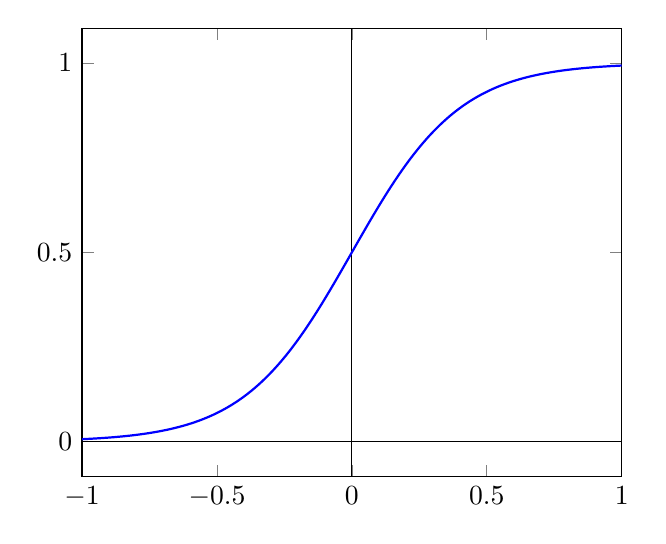
\begin{tikzpicture}
    \begin{axis}[
    	xmin=-1,
        xmax=1,
        ytick distance=0.5
        ]
		\draw[line width=0mm,] 
        (axis cs:\pgfkeysvalueof{/pgfplots/xmin},0) -- 
        (axis cs:\pgfkeysvalueof{/pgfplots/xmax},0);
        
		\draw[line width=0mm] 
        (axis cs:0,\pgfkeysvalueof{/pgfplots/ymin}) -- 
        (axis cs:0,\pgfkeysvalueof{/pgfplots/ymax});

      % plot the stirling-formulae
      \addplot[mark=none, thick, domain=-2:2, blue,samples=500]
      	{1/(1+exp(-5*x))};
    \end{axis}
\end{tikzpicture}

\caption{Sigmoid activation function.}
\label{fig:sigmoid}
\end{figure}

However, close to the end of either sigmoid function, the values of Y respond less to the values of X. In this part, the gradient at that region is really small. This results in a problem known as 'vanishing gradient'. In this part of the curve, the gradient is so small that the neural network cannot learn further. By multiplying such small gradients the values will tend more to zero and thus making the learning process infeasible.

\subsection{Tanh}

Tanh is another function similar to sigmoid. It is also one of the most used activation functions. It also has similar characteristics similar to sigmoid like non-linearity, no activations blowing up and bounded range unlike sigmoid, the range is from (-1, 1).

\begin{equation} \label{eq:tanh}
	f(x)=\frac{\mathrm{2} }{\mathrm{1} + e^{-2x} }-1
\end{equation}

Different from sigmoid, tanh has a stronger gradient this is because the function is steeper. Tanh is useful when a strong gradient is required. Like sigmoid, tanh has the same problem of vanishing gradient. \cite{SharmaVUnderstandingNetworks}

% FIGURE: tanh
\begin{figure}[H]
\centering
\begin{tikzpicture}
    \begin{axis}[
		xmin=-1,
        xmax=1,
        ytick distance=0.5
        ]
		\draw[line width=0mm,] 
        (axis cs:\pgfkeysvalueof{/pgfplots/xmin},0) -- 
        (axis cs:\pgfkeysvalueof{/pgfplots/xmax},0);
        
		\draw[line width=0mm] 
        (axis cs:0,\pgfkeysvalueof{/pgfplots/ymin}) -- 
        (axis cs:0,\pgfkeysvalueof{/pgfplots/ymax});

      % plot the stirling-formulae
      \addplot[mark=none, thick, domain=-2:2, blue,samples=500]
      	{(2/(1+exp(-5*x)))-1};
    \end{axis}
\end{tikzpicture}

\caption{Tanh activation function.}
\label{fig:tanh}
\end{figure}

\subsection{Rectified Linear Units}

In recent years, the use of sigmoid functions such as tanh has dropped in favour of Rectified Linear Units (ReLUs). ReLU function has output 0 if the input is less than 0, and raw output in any other case, equation \ref{eq:relu}. Although a ReLU might seem linear, in fact, it is nonlinear in nature. Combinations of ReLU are also non linear. The range of ReLU is $[0, inf]$, figure \ref{fig:relu}.

\begin{equation} \label{eq:relu}
	f(x)=max(0,x)
\end{equation}

ReLU has been demostrated to make training faster compared to sigmoid or tanh activation functions. Krizhevsky et al. experimented training a Convolutional Neural Network for Imagenet classification with tanh and ReLU activation functions. They showed that the network with ReLU reaches a 25\% training error rate on CIFAR-10 and is six times faster than an equivalent network with tanh neurons \cite{KrizhevskyImageNetNetworks}.

% FIGURE: relu
\begin{figure}[H]
\centering
\begin{tikzpicture}
    \begin{axis}[
    	xmin=-4,
        xmax=4,    
        domain=-3:5,
        ]
		\draw[line width=0mm,] 
        (axis cs:\pgfkeysvalueof{/pgfplots/xmin},0) -- 
        (axis cs:\pgfkeysvalueof{/pgfplots/xmax},0);
        
		\draw[line width=0mm] 
        (axis cs:0,\pgfkeysvalueof{/pgfplots/ymin}) -- 
        (axis cs:0,\pgfkeysvalueof{/pgfplots/ymax});
        
        \addplot+[mark=none,blue,thick,domain=-5:0] {0};
        \addplot+[mark=none,blue,thick,domain=0:5] 	{x};        
    \end{axis}
\end{tikzpicture}

\caption{ReLu activation function.}
\label{fig:relu}
\end{figure}